\documentclass[12pt]{standalone}
\usepackage{tikz}
\usetikzlibrary{patterns} % calc, arrows.meta, decorations.pathreplacing}

\begin{document}

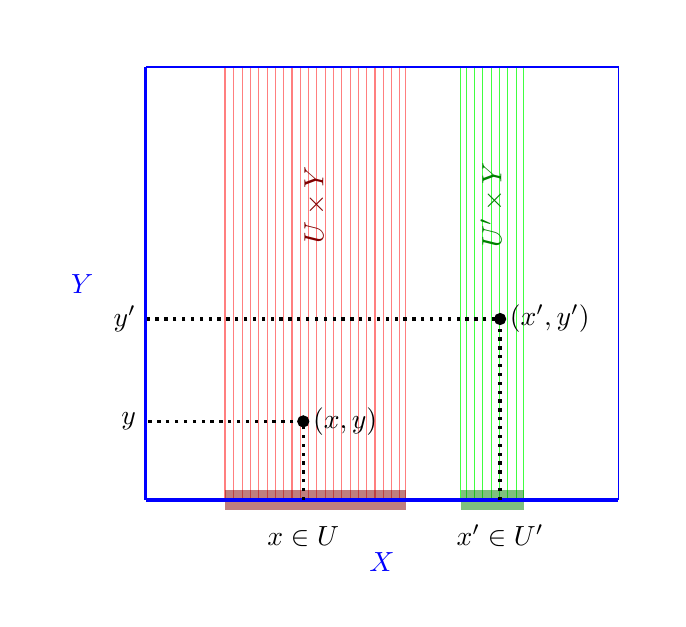
\begin{tikzpicture}
\def\myx{2}
\def\myy{1.5}
\def\myxprime{4.5}
\def\myyprime{2.8}
\path[use as bounding box] (-1.5,-0.75) -- (6.5,-0.75) -- (6.5,6.5) -- (-1.5,6.5) -- cycle; 

	% Draw x and y axes
	%\draw[->] (0,0.5) -- ++(6.5,0); % node[anchor=north] {$x$};
	%\draw[->] (0,0.5) -- ++(0,6); % node[anchor=west] {$y$};

\filldraw[red, pattern=vertical lines, pattern color=red, opacity=0.5] (1,0.5) rectangle (3.3,6);
\node[rotate=90, red!50!black] at (2.15,4.25) {$U\times Y$};
\draw[line width=7pt, opacity=0.5, red!50!black] (1,0.5) -- (3.3,0.5);
\node[anchor=south, yshift=-6pt] at (\myx, 0) {$x\in U$};

	
\filldraw[green, pattern=vertical lines, pattern color=green, opacity=0.75] (4,0.5) rectangle (4.8,6);
\node[rotate=90, green!50!black] at (4.4,4.25) {$U'\times Y$};
\draw[line width=7pt, opacity=0.5, green!50!black] (4,0.5) -- (4.8,0.5);
\node[anchor=south, yshift=-6pt] at (\myxprime, 0) {$x'\in U'$};

	
	\draw[ %-|, 
	very thick, blue] (0,0.5) -- (6,0.5) node[midway, anchor=north, yshift=-15pt]{$X$};
	\draw[ %-|, 
	very thick, blue] (0,0.5) -- (0,6) node[midway, anchor=east, xshift=-15pt]{$Y$};
	\draw[blue] (0,6) -- (6,6) -- (6,0.5);
	
	%\node[anchor=north] at (\myx,0.5) {$x$};
	\node[anchor=east] at (0,\myy) {$y$};
	\draw[dotted, very thick] (\myx,0.5) -- (\myx,\myy) -- (0,\myy);	
	\filldraw (\myx,\myy) circle(2pt) node[anchor=west]{$(x,y)$};

	%\node[anchor=north] at (\myxprime,0.5) {$x'$};
\node[anchor=east] at (0,\myyprime) {$y'$};
\draw[dotted, very thick] (\myxprime,0.5) -- (\myxprime,\myyprime) -- (0,\myyprime);	
\filldraw (\myxprime,\myyprime) circle(2pt) node[anchor=west]{$(x',y')$};


\end{tikzpicture}
\end{document}
